\chapter{Revizuirea Literaturii}

\section{Introducere în EEG}
\subsection{Procesul de recoltare a datelor și aplicații}

\setlength{\abovecaptionskip}{0pt}
\setlength{\belowcaptionskip}{0pt}
\begin{figure}[h]
    \centering
    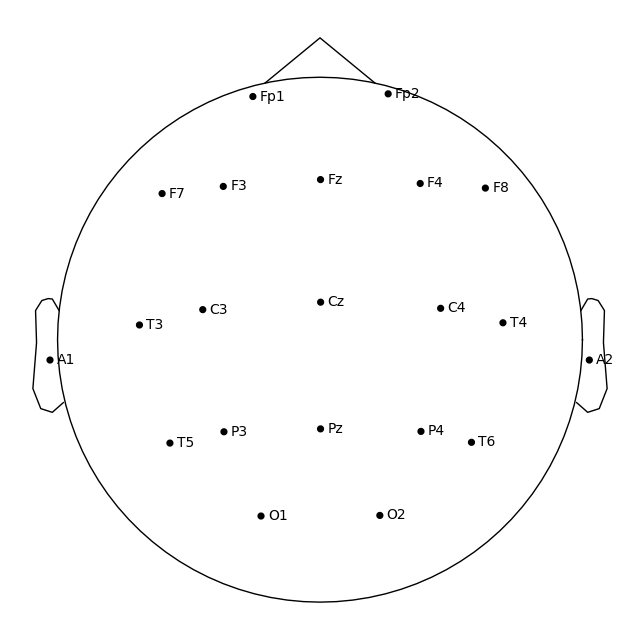
\includegraphics[width=8cm]{images/Sensor_positions_(eeg).png}
    \caption{Pozițiile electrozilor la nivelul capului}
    \label{fig:sensor_positions}
\end{figure}

In total sunt 20 de electrozi. Pz a fost folosit pentru calibrare, deci nu este luat in considerare.

EEG-urile au aplicații intr-o multitudine de domenii. Cele mai folosite cazuri în literatura de specialitate sunt: detectarea fazelor somnului, a simptomelor epilepsiei, a sindromului Alzheimer și, în domeniul de Brain-Computer interface, care se concentrează pe decodarea semnalelor creierului asociate cu mișcarea membrelor

\subsection{Datele recoltate}
Datele recoltate reprezinta 23 de subiecti care ....

\section{Analiza preferințelor umane cu EEG}
\subsection{Cercetări anterioare pe tema preferințelor vizuale.}

\subsection{Tehnologii și abordări existente.}

\section{Tehnologii folosite pentru clasificarea semnalelor EEG}
\subsection{MNE}
\subsection{Braindecode}